\documentclass[conference]{IEEEtran}
\IEEEoverridecommandlockouts
% The preceding line is only needed to identify funding in the first footnote. If that is unneeded, please comment it out.
\usepackage{cite}
\usepackage{amsmath,amssymb,amsfonts}
\usepackage{algorithmic}
\usepackage{graphicx}
\usepackage{textcomp}
\usepackage[table]{xcolor}
\usepackage{xcolor}
\def\BibTeX{{\rm B\kern-.05em{\sc i\kern-.025em b}\kern-.08em
    T\kern-.1667em\lower.7ex\hbox{E}\kern-.125emX}}
\begin{document}

\title{High Level Synthesis Using Genetic Algorithm\\
}

\author{\IEEEauthorblockN{ Andrew Zakhary}
\IEEEauthorblockA{\textit{Electronics Engineering} \\
\textit{Hochschule Hamm-Lippstadt}\\
Hamm, Germany \\
2210009}
}

\maketitle

\begin{abstract}
With electronic components getting smaller and smaller the complexity of the circuitry is growing at an exponential rate. With this came many approaches in simplifying and streamlining the hardware design process. One of these approaches is hardware-software co-design where hardware and software design are interlinked. During this process the software is designed in a way where the hardware can be generated directly from the software design where this is done in formal models or in programming language as SystemC. This approach opened the door to a wide range of algorithms that try to break down the software design and turn it into hardware circuitry in a process called synthesis. In this paper one of these algorithms, namely Genetic Algorithm, is discussed in details and given an example that explains its workings.
\end{abstract}

\begin{IEEEkeywords}
Hardware, Synthesis, hardware software co-design, Genetic algorithm
\end{IEEEkeywords}

\section{Introduction}
Advancements in the VLSI (Very-large-scale integration) technology have made synthesis of electronics circuits using traditional optimization methods for reducing footprint and resources inefficient. As a result, new optimization processes are developed to solve this problem\cite{aminzadeh2006using}.

The synthesis process is responsible for converting the description of the circuit to actual hardware. In broad terms, this is done by achieving two tasks. The fist is scheduling and the second is resource allocation. the scheduling process is responsible for mapping the steps or sub-processes to their clock cycles. This is done while maintaining the dependencies between this process and other processes. Resource allocation however is concerned with mapping the resources needed as registers to save variables, functional units are mapped to logical functions, busses and multiplexers and mapped to interconnections between memory units and functional units\cite{5209958}. As these processes are intertwined an optimized solution must take into account both objectives simultaneously. Thus sequential optimization algorithms can come up short in hardware synthesis. To solve this algorithms like Mixed integer-linear programming can be used. This however becomes impractical very quickly as the cost of generating a solution grow rapidly even for small specifications.\cite{31534}.

Algorithms that are inspired from nature can also be used in this problem as ant colony, genetic algorithm or neural networks as possible solutions to the synthesis problem. Genetic Algorithm (GA) is used extensively in different fields alongside hardware synthesis as AI models, image processing and wireless sensor networks. This is because GA is a general purpose search algorithm that optimizes the intended process according to its fitness function (this will be explained in the upcoming sections). This paper will focus on the application of GA in high level synthesis with a simple example that shows how it is actually implemented in this field.
\section{Basic Concepts}
\subsection{High Level Synthesis}
High level synthesis is a method of generating digital circuits automatically from a behavioral model. This behavioural model  could describe a mathematical equation, the movement of a robot or a home appliance. This behavioral model is usually created in a high level hardware description language (e.g VHDL or Verilog) that is then translated into an intermediate form as a data flow graph (DFG). The DFG shows every process as a separate node running on a specific time slice. Thus scheduling can be directly mapped on the desired DFG and dependencies can be shown by the arrows flowing from one node to another as shown in Fig.\ref{fig:dfg-example}.
\begin{figure}[h]
    \centering
    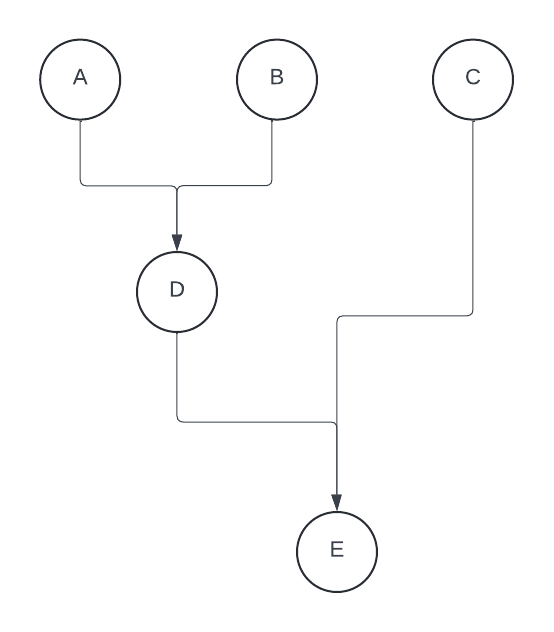
\includegraphics[scale=0.3]{cdfg example.png}
    \caption{Example of a DFG }
    \label{fig:dfg-example} 
\end{figure}
\subsection{Scheduling}
Scheduling such a process can be done in multiple ways. This usually starts by a process to simplify the amount of nodes to be scheduled. One of the simplest and most straight forward methods is the  \textit{mobility analysis}\cite{8252679}. This relies on scheduling the nodes (processes) using ASAP (As Soon As Possible) at one time and then with ALAP(As Late As Possible) next. The difference in time steps for each node is called \textit{mobility} of the node. This makes the scheduling simpler as any node with mobility 0 can't be moved from one variation to another and thus can be eliminated completely from the optimization process. This saves on computation resources needed and the time as well which in larger and more complex algorithms rather critical.

This has some limitations though, one of the assumptions of this method is that it assumes infinite resources. As with ASAP for example, all available processes are run at the same time slot. In reality however, this is often not the case, where the systems can be constrained by a maximum number of registers, Functional Units, ALUs , etc. This can be mitigated by analyzing on \textit{availability} basis. This is applied by constantly checking the available nodes according their dependencies \textbf{and} the availability in resources. As a consequence this makes the scheduling process more complex due to the loss of ability to eliminate nodes ahead of time as is done in mobility analysis.
\subsection{Genetic Algorithm}
Over the years, biology has inspired technology in many different ways. After all, life has found multitude of ways to exist and persist over billions of years in an always changing environmental conditions. Also, as resources in nature are limited there's a constant competition on them, out of this competition arises a constant need for improvement and efficiency. One of the aspects of nature that has been used extensively in the tech sector is the Genetic Algorithm (GA). GA in nature is performed by two main processes. These are: 
\begin{itemize}
    \item \textbf{Evolution} This is the change that happens to the traits of the individuals from one generation to another. These changes in most cases can be very small and not even visible but the accumulation of these changes can cause dramatic changes over time.
    \item \textbf{Natural selection} This is the rule that since resources are limited, the survival is only available to the fittest individuals and the most suitable to their environment.
\end{itemize}
These two processes work together resulting in an optimization search for the fittest individuals in the population that can breed and generate another generation that because of the same processes would be even fitter. The evolution process generates these changes based on another two processes\cite{681007} which are :
\begin{itemize}
    \item \textbf{Cross-Over} This is process where the two sets of chromosomes (i.e traits) of the parents and mixed and matched to generate a single set of chromosomes that would be inherited by their offspring.
    \item \textbf{Mutation} This is a process where the chromosomes (traits) of the offspring are changed randomly.
\end{itemize}
these two processes work together to make sure that there's always a replenishing new set of traits being generated in the genetic pool.

These individuals are then governed by the law of natural selection. As the resources available are limited, this law describes how the survival of the offsprings is always contingent on them being more fit for their environment. With the creation processes mentioned before this inevitably leads to the permeation of specific traits. These traits are mostly only changed with the change the environment.
\section{Implementation}

\subsection{Methodology}

Implementing GA in High Level Synthesis is done by simulating individuals of a population as solutions to the scheduling/resource allocation problem. This can be done by showing each individual as a table where each column corresponds to a time slot and each row corresponds to a resource being allocated. Firstly these individuals can be generated at random whether by mobility analysis or availability analysis depending on the available resources. Then natural selection needs to be simulated\cite{daalder1996high}. This is done by the means of a fitness function that grades each individuals. This is left to the designer of the system. This freedom in designing is the whole reason why GA is very powerful. The fitness formula can be designed to fit any number of resources needed to be optimized. Not only that, but it can also have different weights for the different optimized resources. 

After the first generation generation is created and graded comes the step of selecting the best fitting individuals and \textit{breeding} them in order to create a new generation built on the traits of the best performing parents. The creation of this generation can be done in different ways. One of these is slicing and matching, this is done by matching where the two parents have similar traits and seeing where the traits differ and mixing traits from the two parents. This generation is then graded using the fitness formula used for the previous generation and the process repeats.

In the following section we take a look at an example of HLS using the GA. This example is simplifying the process by only analyzing ALUs as the resources in concern.
\subsection{Example}
Assume a system of differential equations described by the following HDL code :
\begin{verbatim}
module diffEqn (x, dx, u, a, clock, y)
input x, dx, u, a, clock;
output y;
always @(posedge clock)
    while (x<a)
        begin
        x1=x+dx;
        u1=u-(3*x*u*dx)-(3*y*dx);
        y1=y+(u*dx);
        x=x1;
        u=u1;
        y=y1;
        end
endmodule
\end{verbatim}
A control data flow graph (CDFG) can be generated for the process as shown in Fig.\ref{fig:CDFG}. This shows the different operations (multuplications,comparisons, addition and subtraction). The inputs could be removed from the top layer, and processes given names in order to make it more readable as shown if Fig.\ref{fig:cdfg_cleaned}
\begin{figure}[h]
    \centering
    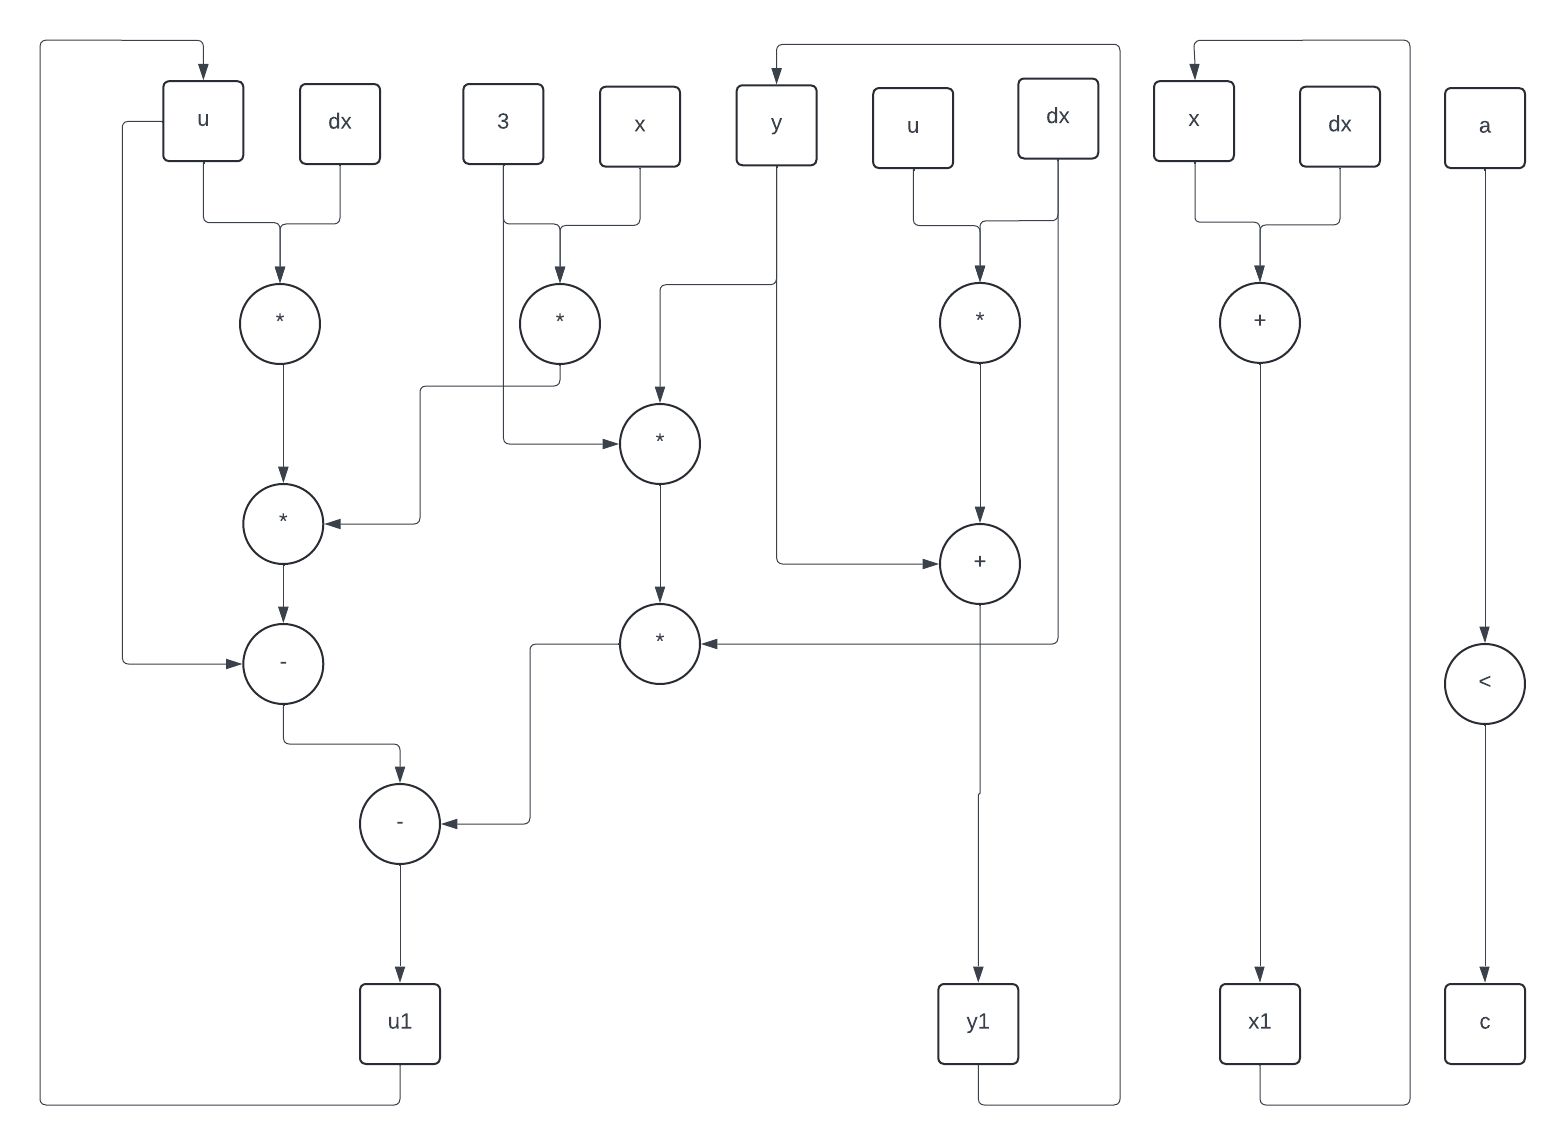
\includegraphics[scale=0.3]{cdfg.png}
    \caption{CDFG for second order differential equation}
    \label{fig:CDFG}
\end{figure}
\begin{figure}[h]
    \centering
    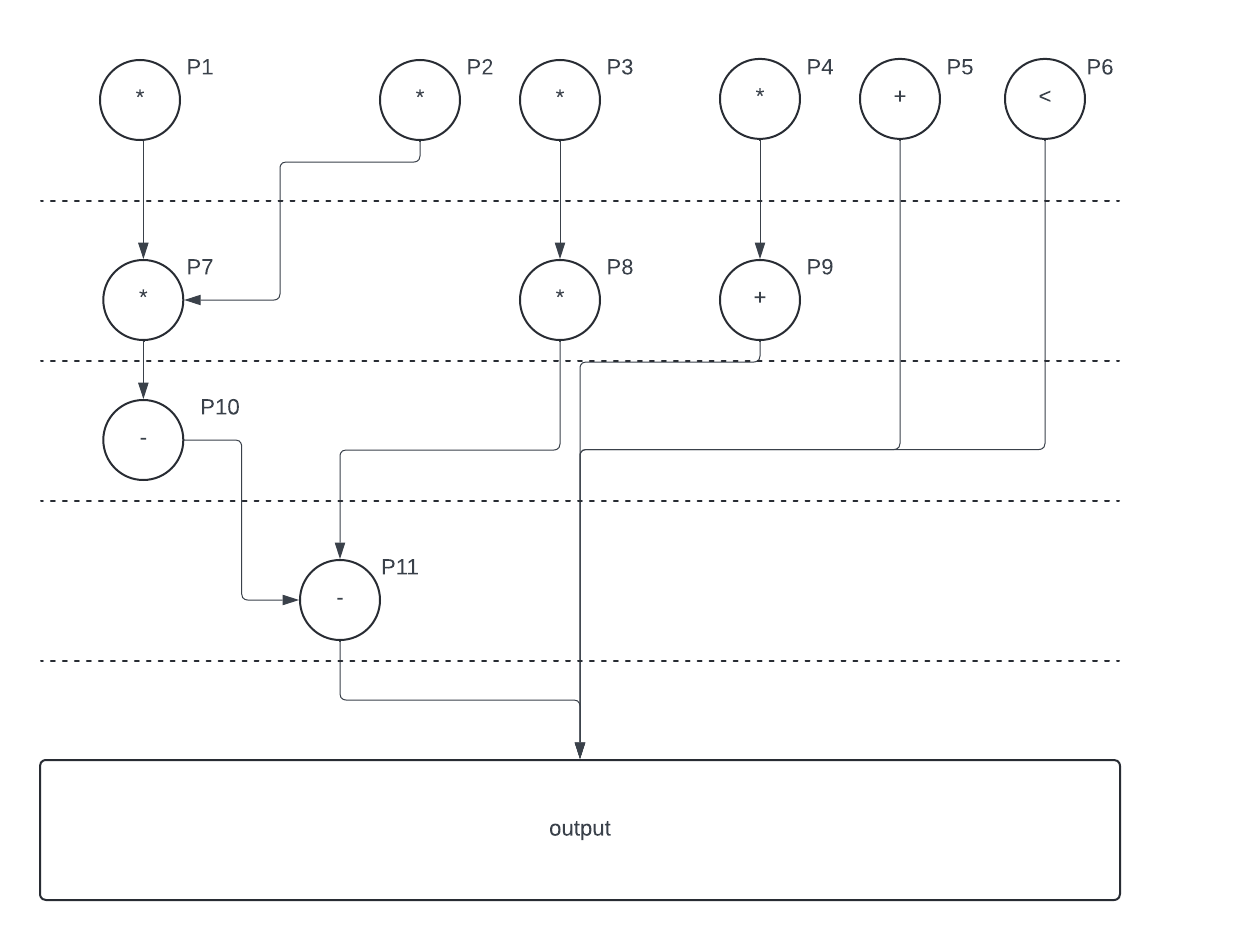
\includegraphics[scale=0.4]{CDFG CLEANED.png}
    \caption{Cleaned CDFG diagram}
    \label{fig:cdfg_cleaned}
\end{figure}

As can be visualized from Fig.\ref{fig:cdfg_cleaned}, some processes need other processes to be completed before they can be run themselves. This condition is called \textit{Dependency} and it is very important in hardware synthesis. As multiple solutions will be proposed in the upcoming section will be presented, it is very important to be able to check if the dependencies are met or not. For this Table\ref{tab:Dependencies} is created to easily check if dependencies are met.
\begin{table}
    \centering
    \begin{tabular}{|c|c|}
    \hline
       Dependent process  & Dependent on \\
       \hline \hline
       $P7$  &  $P1,P2$ \\
       \hline
        $P8$ & $P3$ \\
        \hline
       $P9$ & $P4$ \\
       \hline
       $P10$ & $P7$ \\
       \hline
       $P11$ & $P10,P8$ \\
       \hline
    \end{tabular}
    \vspace{2pt}
    \caption{Dependencies table}
    \label{tab:Dependencies}
\end{table}

To better visualize the power of genetic algorithm as searching algorithm in such a simple example it's wise to constrain the resources of the hardware to be designed in order to get a wider variety of the population generated. For this example a constraint of only 3 ALUs are assumed. This means since our focus is on the mathematical operations in the code, the solutions are limited to three operations in parallel in each clock cycle. In this example other operations (e.g reading from memory, writing to memory, sending control signals,.. etc) are not calculated as they are assumed similar in all proposed solutions. In practice this might not be the case depending on the program to be designed in hardware.

The fitness formula used in this example is proposed to be the utilization of the 3 ALUs available during the program run time as shown in the equation (\ref{rho_1}). As every process is done on a single ALU, it is assumed each process only takes one clock cycle. This makes the total runtime of the ALUs fixed to 11 units of time the program has 11 processes.
\begin{equation}
    \rho=\Sigma\frac{T_{ALU}}{T_{Total}}=\frac{11}{T_{Total}}
    \label{rho_1}
\end{equation}
With this explained the creation of the first generation can start. Each Individual will be created in a separate table and their fitness will be compared afterwards.
\begin{table}[h!]
    \centering
    \begin{tabular}{|c|c|c|c|c|c|c|}
    \hline
    ALU \#  & $T_1$ & $T_2$ &  $T_3$& $T_4$ & $T_5$ & $T_6$\\
    \hline
       ALU \#1  & P4 & P2 &  P1& P7 & P10 & P11\\
       \hline
       ALU \#2  &  P5 & P3 & P8 &  &  & \\
       \hline
       ALU \#3  & P6 & P9  &  &  &  & \\
       \hline
    \end{tabular}
           \vspace{2pt}
    \caption{Individual \#1}
    \label{tab:Individual1}
\end{table}
\begin{table}[h!]
    \centering
    \begin{tabular}{|c|c|c|c|c|c|c|}
        \hline
    ALU \#  & $T_1$ & $T_2$ &  $T_3$& $T_4$ & $T_5$ & $T_6$\\
    \hline
       ALU \#1  & P3 & P8 &  P1& P7 & P10 & P11\\
       \hline
       ALU \#2  &  P4 & P9 & P2 &  &  & \\
       \hline
       ALU \#3  & P5 & P6  &  &  &  & \\
       \hline
    \end{tabular}
           \vspace{2pt}
    \caption{Individual \#2}
    \label{tab:Individual2}
\end{table}
\begin{table}[h!]
    \centering
    \begin{tabular}{|c|c|c|c|c|c|}
        \hline
    ALU \#  & $T_1$ & $T_2$ &  $T_3$& $T_4$ & $T_5$ \\
    \hline
       ALU \#1  & P1 & P7 &  P3& P8 & P11\\
       \hline
       ALU \#2  &  P2 & P9 & P6 &  &\\
       \hline
       ALU \#3  & P4 & P5  & P10 &  & \\
       \hline
    \end{tabular}
           \vspace{2pt}
    \caption{Individual \#3}
    \label{tab:Individual3}
\end{table}
\begin{table}[h!]
    \centering
    \begin{tabular}{|c|c|c|c|c|c|}
    \hline
    ALU \#  & $T_1$ & $T_2$ &  $T_3$& $T_4$ & $T_5$ \\
        \hline
       ALU \#1  & P1 & P7 &  P9& P8 & P11\\
       \hline
       ALU \#2  &  P2 & P4 & P6 &  &\\
       \hline
       ALU \#3  & P3 & P5  & P10 &  & \\
       \hline
    \end{tabular}
           \vspace{2pt}
    \caption{Individual \#4}
    \label{tab:Individual4}
\end{table}

\begin{table}[h!]
    \centering
    \begin{tabular}{|c|c|c|c|c|}
    \hline
        Individual & \#1 & \#2 & \#3 & \#4\\
        \hline
        Fitness & 61.11\% & 61.11\% & 73.33\% & 73.33\%\\
        \hline
    \end{tabular}
    \vspace{2pt}
    \caption{Fitness comparison}
    \label{tab:fitness}
\end{table}

By comparing the first generation that was randomly created, the highest rated individuals can be selected in order to create the second generation's offspring. According to table\ref{tab:fitness} Individuals \#3 and \#4 are selected. In order to do so, it is necessary to see where slices and matches can be done. This can be visualized by color coding the individuals' similarities and dissimilarities. In the tables below the similarities are highlighted by the green color, while the differences are highlighted by the orange and blue colors for individuals  \#3 and \#4 respectively as shown in Tables \ref{tab:Individual3-colored} and \ref{tab:Individual4-colored}. 
\begin{table}[h!]
    \centering
    \begin{tabular}{|c|c|c|c|c|c|}
        \hline
    ALU \#  & $T_1$ & $T_2$ &  $T_3$& $T_4$ & $T_5$ \\
    \hline
       ALU \#1  &\cellcolor[HTML]{51C004} P1 &\cellcolor[HTML]{51C004} P7 &\cellcolor[HTML]{D67D03}  P3& \cellcolor[HTML]{51C004}P8 & \cellcolor[HTML]{51C004}P11\\
       \hline
       ALU \#2  &  \cellcolor[HTML]{51C004}P2 & \cellcolor[HTML]{D67D03}P9 & \cellcolor[HTML]{51C004}P6 &  &\\
       \hline
       ALU \#3  &\cellcolor[HTML]{D67D03} P4 & \cellcolor[HTML]{51C004}P5  & \cellcolor[HTML]{51C004}P10 &  & \\
       \hline
    \end{tabular}
           \vspace{2pt}
    \caption{Individual \#3}
    \label{tab:Individual3-colored}
\end{table}
\begin{table}[h!]
    \centering
    \begin{tabular}{|c|c|c|c|c|c|}
    \hline
    ALU \#  & $T_1$ & $T_2$ &  $T_3$& $T_4$ & $T_5$ \\
        \hline
       ALU \#1  & \cellcolor[HTML]{51C004}P1 &\cellcolor[HTML]{51C004} P7 & \cellcolor[HTML]{0079EA} P9&\cellcolor[HTML]{51C004} P8 &\cellcolor[HTML]{51C004} P11\\
       \hline
       ALU \#2  & \cellcolor[HTML]{51C004} P2 &\cellcolor[HTML]{0079EA} P4 & \cellcolor[HTML]{51C004}P6 &  &\\
       \hline
       ALU \#3  &\cellcolor[HTML]{0079EA} P3 & \cellcolor[HTML]{51C004}P5  &\cellcolor[HTML]{51C004} P10 &  & \\
       \hline
    \end{tabular}
           \vspace{2pt}
    \caption{Individual \#4}
    \label{tab:Individual4-colored}
\end{table}

Using these two individuals as parents to the next generation, the Cross-over process can simulated by randomly swapping the differences while keeping the similarities the same. In this example two offsprings are generated by swapping the differences one at a time as shown in Tables \ref{tab:offspring-1} and \ref{tab:offspring-2}.

\begin{table}[h!]
    \centering
    \begin{tabular}{|c|c|c|c|c|c|}
        \hline
    ALU \#  & $T_1$ & $T_2$ &  $T_3$& $T_4$ & $T_5$ \\
    \hline
       ALU \#1  &\cellcolor[HTML]{51C004} P1 &\cellcolor[HTML]{51C004} P7 & P9& \cellcolor[HTML]{51C004}P8 & \cellcolor[HTML]{51C004}P11\\
       \hline
       ALU \#2  &  \cellcolor[HTML]{51C004}P2 & P3 & \cellcolor[HTML]{51C004}P6 &  &\\
       \hline
       ALU \#3  & P4 & \cellcolor[HTML]{51C004}P5  & \cellcolor[HTML]{51C004}P10 &  & \\
       \hline
    \end{tabular}
           \vspace{2pt}
    \caption{Offspring \#1}
    \label{tab:offspring-1}
\end{table}
\begin{table}[h!]
    \centering
    \begin{tabular}{|c|c|c|c|c|c|}
    \hline
    ALU \#  & $T_1$ & $T_2$ &  $T_3$& $T_4$ & $T_5$ \\
        \hline
       ALU \#1  & \cellcolor[HTML]{51C004}P1 &\cellcolor[HTML]{51C004} P7 & P4&\cellcolor[HTML]{51C004} P8 &\cellcolor[HTML]{51C004} P11\\
       \hline
       ALU \#2  & \cellcolor[HTML]{51C004} P2 & P9 & \cellcolor[HTML]{51C004}P6 &  &\\
       \hline
       ALU \#3  & P3 & \cellcolor[HTML]{51C004}P5  &\cellcolor[HTML]{51C004} P10 &  & \\
       \hline
    \end{tabular}
           \vspace{2pt}
    \caption{Offspring \#2}
    \label{tab:offspring-2}
\end{table}
By analyzing the two offsprings, it is noticed that the the fitness stays the same at $\frac{11}{15}$ or $73.33\%$. By analyzing the dependencies mentioned in Table \ref{tab:Dependencies} however, it is noticed that Offspring \#2 has the process P9 at time $T_2$ before executing P4 at time $T_3$. In Genetic Algorithm such cases can happen where even though both parents offer valid solutions this doesn't necessarily mean that their offspring must be also a valid solution.

As shown the cross-over process alone retains the majority of the traits of the parents specially if they are fairly similar as in the example given. This is where the Mutation process plays a big role. It introduces random changes that has the ability to break the pattern of the traits had by both parents and introduces new traits. In practicality Mutation's contributions are almost always very small and in search algorithms as GA it can introduce a lot of invalid traits as it is random by nature. The inclusion of such invalid offsprings is a design choice as similar to how valid parents can give birth to invalid offsprings, invalid parents can give birth to valid offsprings. This process however needs a lot of time, larger sized populations and algorithms to check the validity of each offpsring.

In this example a mutation can be simulated by swapping the execution of P8 at $T_4$ with P5 at $T_2$ in individual \#4 which results in The dependency of the process P11 to be done earlier. This allows the parallelism  of the process P5 and P11 saving a complete clock cycle as shown in Table \ref{tab:mutated} with the mutated processes shown in red.
\begin{table}[h!]
    \centering
    \begin{tabular}{|c|c|c|c|c|}
        \hline
    ALU \#  & $T_1$ & $T_2$ &  $T_3$& $T_4$ \\
    \hline
       ALU \#1  &\cellcolor[HTML]{51C004} P1 &\cellcolor[HTML]{51C004} P7 & \cellcolor[HTML]{0079EA} P9& \cellcolor[HTML]{E60000}P5 \\
       \hline
       ALU \#2  &  \cellcolor[HTML]{51C004}P2 &\cellcolor[HTML]{0079EA}  P4 & \cellcolor[HTML]{51C004}P6 & P11 \\
       \hline
       ALU \#3  &\cellcolor[HTML]{0079EA} P3 & \cellcolor[HTML]{E60000}P8  & \cellcolor[HTML]{51C004}P10 &  \\
       \hline
    \end{tabular}
           \vspace{2pt}
    \caption{Mutated offspring \#3}
    \label{tab:mutated}
    \end{table}

Analyzing the fitness of offspring \#3 it is seen that it reached 91.67\% which in this case is the maximum utilization possible for a solution with the constrain of 3 ALUs assumed at the beginning of the example.

\section{Conclusion}
Genetic Algorithm has definitely proved itself as an important search algorithm in multiple applications and specially in High Level Synthesis. The algorithm can reach optimized solutions with competitive accuracy and with built in methods that would get out of local optima. In larger and more complex scenarios the generation of sufficiently enough populations can be demanding in regards of resources but this can cut the amount of generations needed to reach an optimized solution which subsequently would lessen the run time. On the other side however adjusting the parameters for things like mutations rate and crossover percentages can be very tricky as the algorithm is very sensitive to such changes. It is also worth mentioning that the fitness formula is of upmost priority when designing a GA. All in all the GA has been used for a long time and there's no signs of this not continuing in the future as the concepts it's built upon are also still in action every day in the biology happening all around.
\bibliographystyle{unsrt} 
\bibliography{refs}

\end{document}
